\section{Selection of tags}
\label{sec:tags}

The definition of tags and trees of tags will be presented subsequently for the dynamic environment, for the static environment, and finally for the conditions.



\subsection{Tags for the dynamic environment}
\label{sec:selection of tags dynamic}

To describe the dynamic environment, the activities of the different actors are described. First, we consider different type of actors in \cref{sec:type of actor}. Next, in \cref{sec:activities}, tags are provided to describe the activities of the actors. In \cref{sec:initial state}, tags are presented that describe the initial state of an actor in a scenario. Some special tags are applicable for vehicle driving in front of the ego vehicle, see \cref{sec:lead vehicle}. %We end this section with few tags for animals.



\subsubsection{Carriageway user type}
\label{sec:type of actor}

A first distinction within a scenario is usually made for the type of carriageway user, see \cref{fig:tree carriageway user type}. The tree of tags is not considered to be complete, however, the current tags cover the most common type of carriageway users. For the motorized vehicle a reference is made to the UNECE regulation \autocite{UNECE2011consolidated}. In the regulation, a further distinction in vehicle categories is made. The more general tag ``vehicle'' applies if a vehicle could be either of category M, N, or L. For the category of Vulnerable Road Users (VRU), the European convention is used, with the exception that powered two wheelers, such as a motorcycle, are explicitly considered a vehicle and not a VRU. The reason to use the separate category L, i.e., motor vehicles with less than four wheels, is the large difference in behavior they exhibit compared to VRU; their position on the road and their riding dynamics including speed are just two of the striking differences. 

\begin{figure*}[t]
	\centering
	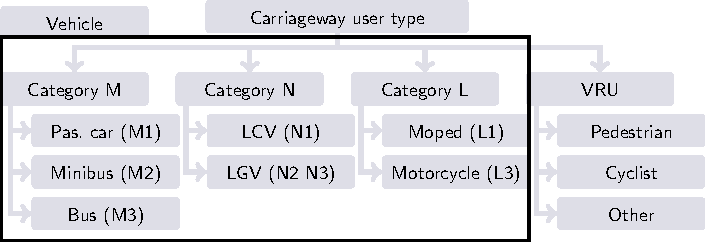
\includegraphics{figures/actor_type}
	\caption{Tags for the type of the carriageway user, with a reference to UNECE vehicle categories \autocite{UNECE2011consolidated}. %Category M refers to power-driven vehicles having at least four wheels and used for the carriage of passengers. Category N refers to power-driven vehicles having at least four wheels and used for the carriage of goods. Category N consists of the subcategories light commercial vehicle (LCV) and large goods vehicle (LGV). Category L refers to motor vehicles with less than four wheels. 
		A vehicle of category M, N, or L is considered as a \emph{vehicle} in the context of this report as indicated by the black box outline. 
		%Note that the list is not complete. For a full reference, see \cite{vehicle_categories2011}.
	}
	\label{fig:tree carriageway user type}
\end{figure*}



\subsubsection{Activities}
\label{sec:activities}

An activity describes the behavior related to an actor. This includes, but is not limited to, the dynamic driving tasks as mentioned in SAE J3016 \cite{sae2018j3016}. In this paper, only the lateral motion control (via steering) and longitudinal motion control (via acceleration and deceleration) are reflected into tags.

The lateral and longitudinal activities of the a vehicle are characterized by the tags of \cref{fig:activities}. The tags may also refer to the objective of the ego vehicle in case no activities are defined. For example, a test case in which the ego vehicle's objective is to make a left turn, the tags ``Turning'' and ``Left'' are applicable. 

\begin{figure*}[t]
	\centering
	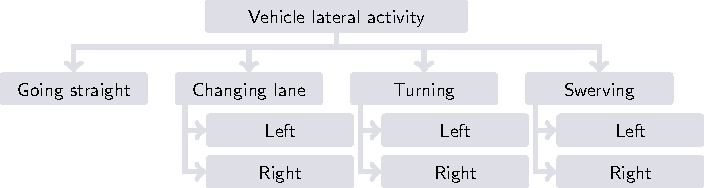
\includegraphics{figures/lat_activity}\\
	\vspace{0.5em}
	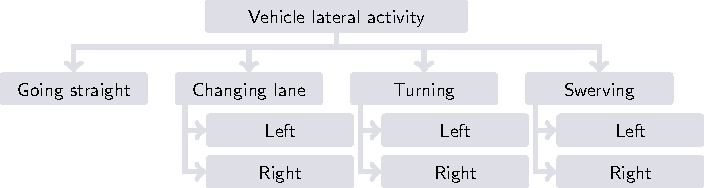
\includegraphics{figures/lat_activity}
	\caption{Tags for lateral and longitudinal activities of a vehicle. 
		%The lateral activity is relative to the lane in which the corresponding vehicle is driving. For example, if the vehicle is driving on a curved road, its lateral activity is ``Going straight''. 
		%As shown in \cref{fig:tree carriageway user type}, the term vehicle could refer to a car, truck/bus, or powered two wheeler.
	}
	\label{fig:activities}
\end{figure*}

Four different types of activities are identified regarding the lateral movement. Here, it is assumed that ``Lateral'' refers to the direction perpendicular to the lane the vehicle is driving in. Therefore, if the vehicle is driving on a curved road while staying more or less in its lane (lane following), the tag ``Going straight'' is applicable. When the vehicle changes lane to an adjacent lane, the tag ``Changing lane'' is applicable. The tag ``Turning'' is applicable when the vehicle turns at a junction. The tag ``Swerving'' is applicable when the vehicle significantly changes lateral position without performing a complete lane change. For example, when the vehicle overtakes a cyclist that is riding at one side of the lane, the vehicle might swerve to the other side of the lane. 

Three different types of activities are identified regarding the longitudinal movement. A distinction is made between driving forward, reversing, and standing still. Regarding driving forward, a further distinction is made with respect to the acceleration.

Due to the typical dynamics for pedestrians and cyclists, separate tag trees are envisioned to characterize their behavior. However, for the sake of brevity, the actual trees are omitted here. We refer the interested reader to \autocite{degelder2019scenariocategories} where we also present these tag trees.
%Due to the pedestrian's specific dynamics, no separate lateral and longitudinal activities are distinguished. A distinction is made between ``Walking'', ``Stopping'' and ``Standing still'', a distinction is made in walking ``Straight'', ``Turning left'', or ``Turning right''. Furthermore, a pedestrian can almost instantaneously come to a full stop (hence the tag ``Stopping'') and can be ``Standing still''. Similar to large deceleration levels for stopping, large acceleration levels can be deployed to start walking. 
%\begin{figure*}
%	\centering
%	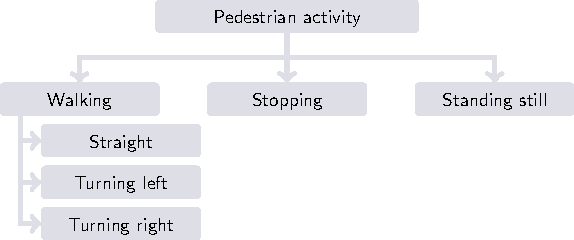
\includegraphics{figures/ped_activity}
%	\caption{Tags for pedestrian activities.}
%	\label{fig:tree pedestrian act}
%\end{figure*}
%
%\Cref{fig:tree cyclist lat act,fig:tree cyclist long act} show the typical activities for a cyclist. For cyclists, a distinction between lateral and longitudinal activities is made, similar to the distinction for vehicles. In the same way as for pedestrians, a tag for both ``Stopping'' and ``Standing still'' is used. As a cyclist can exhibit high deceleration levels, a differentiation is made between a forceful deceleration until standstill (Stopping) and the activity of being at standstill.
%
%\begin{figure*}
%	\centering
%	\begin{subfigure}{\linewidth}
%		\centering
%		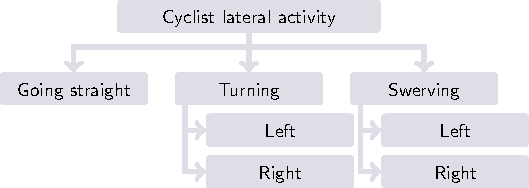
\includegraphics{figures/cyc_lat_activity}
%		\caption{\vspace{0.5cm}}
%		\label{fig:tree cyclist lat act}
%	\end{subfigure}
%	\begin{subfigure}{\linewidth}
%		\centering
%		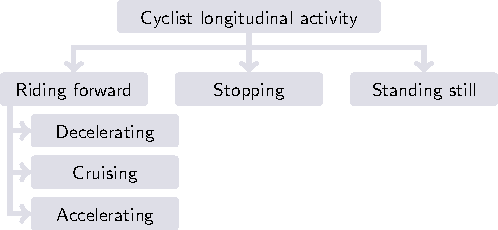
\includegraphics{figures/cyc_lon_activity}
%		\caption{}
%		\label{fig:tree cyclist long act}
%	\end{subfigure}
%	\caption{Tags for cyclist lateral and longitudinal activities.}
%\end{figure*}
%
%Note that other types of actors, such as mono-wheels and powered skateboards, can also have their trees of tags that characterize their behaviour. Because these types of actors are not yet explicitly included into the scenario categories in \cref{sec:categories}, no special tags describing their activities are defined in this report.



\subsubsection{Initial state}
\label{sec:initial state}

\Cref{fig:tree initial state} shows tags for the initial state of the potential other road users with respect to the ego vehicle. A distinction is made in the initial direction of orientation of the road user, the initial dynamics, and the initial longitudinal and lateral position. Three tags, i.e., ``Same as ego'', ``Oncoming'', and ``Crossing'', refer to the initial direction of the road user with respect to the initial direction of the ego vehicle. %Obviously, the tag ``Same as ego'' refers to road users that are oriented in the same direction as the ego vehicle. The tag ``Oncoming'' refers to road users that approach the ego vehicle from the opposite direction. For the other road users, the tag ``Crossing'' is applicable.
The tag ``Dynamics'' refers to the initial dynamics of the road user; the tag distinguishes between initially moving and standing still at the start of the scenario. 
Finally, two tags are used to describe the initial position of the actor with respect to the ego vehicle, in longitudinal and lateral direction. 

\begin{figure*}[t]
	\centering
	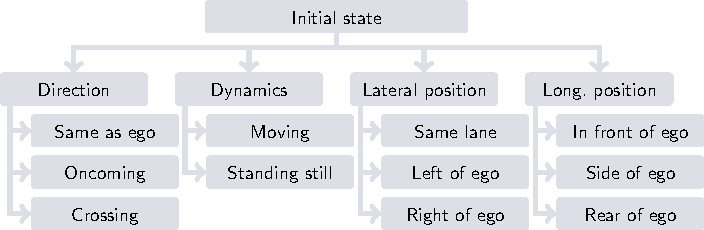
\includegraphics{figures/initial_state}
	\caption{Tags regarding the initial position and movement of road users in a scenario.}
	\label{fig:tree initial state}
\end{figure*}

%Note that the relative direction of a road user might change during the course of a scenario. For example, a vehicle that approaches from the left of the ego vehicle will drive in the same direction as the ego vehicle if it turns left while the ego vehicle continues to drive straight and does not change its direction. To avoid ambiguity, the tags, describing the relative position and activities of road users, refer to the initial position and movement of the corresponding road user with respect to the initial position and movement of the ego vehicle. 
%A distinction is made between road users approaching from the left side (nearside in Singapore) and from the right side (farside in Singapore). There are several reasons to make the distinction between a nearside or farside approach:
%
%\label{page:reasons for distinction far and near}
%\begin{itemize}
%	\item Rules for giving way are different for the near- and farside.
%	\item The setup of an AV is possibly not symmetric with respect to the left and right direction. Even when the AV has been designed to be symmetric, it might not behave symmetrically. When the AV correctly responds to a crossing actor from the nearside, it is not guaranteed that it responds equally correctly to a crossing actor from the farside.
%	\item The response time for actors approaching from the nearside and the farside is different, as actors from the farside first usually need to cross at least one lane before interfering with the path of the ego-vehicle.  
%\end{itemize}
%Multiple tags can be applicable for a scenario. For example, if there is a vehicle driving in front of the ego vehicle and there is a vehicle overtaking the ego vehicle on the right lane, the tags (``Same direction'', ``Same lane'') and (``Same direction'', ``Right of ego'') are applicable. 

%Similar to the tree of tags for vehicles, there are trees for cyclists and pedestrians, see \cref{fig:tree target cyclist,fig:tree target pedestrian}, respectively.

%\begin{figure}
%	\centering
%	\tree{Cyclist initial state}{Oncoming,Left of ego,Same lane, Right of ego;Same direction,Left of ego,Same lane,Right of ego;Crossing,Left,Right;Stationary}
%	\caption{Tags regarding the initial position and movement of cyclists in a scenario.}
%	\label{fig:tree target cyclist}
%\end{figure}
%\begin{figure}
%	\centering
%	\tree{Pedestrian initial state}{Oncoming,Left of ego,Same lane, Right of ego;Same direction,Left of ego,Same lane,Right of ego;Crossing,Left,Right;Stationary}
%	\caption{Tags regarding pedestrians in a scenario.}
%	\label{fig:tree target pedestrian}
%\end{figure}



\subsubsection{Lead vehicle}
\label{sec:lead vehicle}

\Cref{fig:tree lead vehicle} contains the tags that are specifically related to a lead vehicle, i.e., a vehicle that is driving directly in front of the ego vehicle. Two different ways of an appearing lead vehicle are considered. The tag ``Cutting-in'' refers to a vehicle that changes lane such that it ends at the ego vehicle's lane and a ``Gap-closing'' refers to a vehicle that is already in the ego vehicle's lane and appears in the ego vehicle's field of view. In a similar manner, two different ways of a disappearing lead vehicle are considered, ``Cutting-out'' and ``Gap-opening'' respectively. An additional tag ``Following'' is added to describe the situation that the ego vehicle is continuously following the lead vehicle for the duration of a scenario.

\begin{figure}
	\centering
	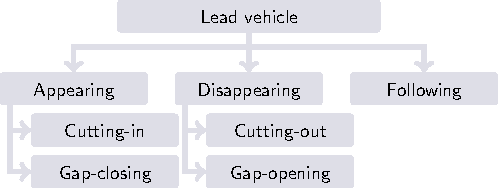
\includegraphics{figures/lead_vehicle}
	\caption{Tags for a lead vehicle, i.e., a vehicle driving in front of ego vehicle.}
	\label{fig:tree lead vehicle}
\end{figure}

%Note that the tags related to lead vehicle are used to emphasize the role of an actor in a scenario. For example, a vehicle that is initially driving in the same direction as the ego vehicle, in the same lane as the ego vehicle, and in front of the ego vehicle (see \cref{fig:tree initial state}) is not necessarily a lead vehicle. In other words, the tags that are earlier presented are not sufficient for expressing the role of lead vehicle.



%\subsubsection{Animals}
%\label{sec:animals}
%
%The presence of animals in the scenario can be described using the tags shown in \cref{fig:tree animals}. 
%
%\begin{figure}
%	\centering
%	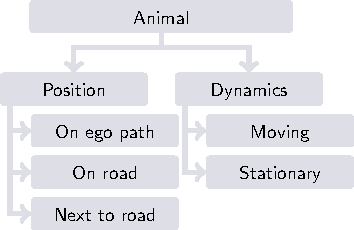
\includegraphics{figures/animal}
%	\caption{Tags that describe the presence of animals.}
%	\label{fig:tree animals}
%\end{figure}



\subsection{Tags for the static environment}
\label{sec:tags selection static}

In this paper, we consider for the static environment the road type (\cref{sec:road type}), the road layout (\cref{sec:road layout}), static objects (\cref{sec:static object}), and a traffic light (\cref{sec:traffic light}).



\subsubsection{Road type}
\label{sec:road type}

The tags for the road type on which the ego vehicle is driving are based on the classification that OpenStreetMaps uses \autocite{HighwayKeyOSM}. We omit the tree of tags because of limited space. We refer the interested reader to \autocite{HighwayKeyOSM}

% see \cref{fig:tree road type}. A distinction is made between principal roads and link roads. The link roads refer to roads that are leading to or from the specified road type from or to the specified road type or a lower class road type \cite{HighwayKeyOSM}. Here, a lower class road type refers to all road types listed below the specified road type in \cref{fig:tree road type}. For example, the ``Trunk link'' refers to a road leading to or from a trunk road from or to a road type listed below ``Trunk'' in \cref{fig:tree road type}.
%
%\begin{figure}
%	\centering
%	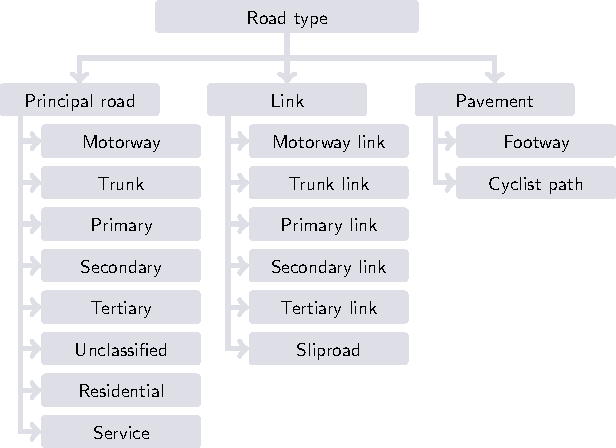
\includegraphics[width=\linewidth]{figures/road_type.pdf}
%	\caption{Tags for the type of road, based on the highway tag used for OpenStreetMaps \cite{HighwayKeyOSM}.}
%	\label{fig:tree road type}
%\end{figure}



\subsubsection{Road layout}
\label{sec:road layout}

The layout of the road is specified using the tags in \cref{fig:tree road layout}. Here, four categories are defined. Typically, highway roads will mainly be in the category ``Straight''. The second subcategory, i.e., ``Curved'', refers to roads that are highly curved. Typically, the actual speed to safely and comfortably drive these curved roads is lower than the speed limit on the straight section preceding the curved road. For example, a curved road right after a highway exit can often be classified as ``Curved''. The other two categories refer to junctions, whereas ``Pedestrian crossing'' refers to intersections where only a footway is intersecting with the road the ego vehicle is driving on, e.g., a zebra crossing. A large roundabout may be regarded as multiple junctions that are close to each other. For smaller roundabouts, it might be better to treat the roundabout as a whole instead of treating it as multiple junctions. In that case, the ``Roundabout'' tag applies.

\begin{figure*}[t]
	\centering
	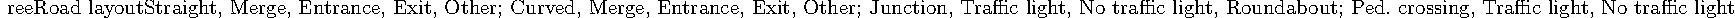
\includegraphics{figures/road_layout}
	\caption{Tags that describe the road layout.}
	\label{fig:tree road layout}
\end{figure*}



\subsubsection{Static object}
\label{sec:static object}

The presence of static objects are described using the tags presented in \cref{fig:tree static object}. A distinction is made between objects that are on the intended path of the ego vehicle and objects that are not on the intended path but are still of importance as they might be blocking the view of the ego vehicle. When a static object is on the intended path of the ego vehicle, the object might be passable - when it is possible to drive over it, or impassable - when the ego vehicle can only avoid undesired interaction with the object by steering around it.

Strictly speaking, every object that is in the field of view of the ego vehicle is blocking part of the ego vehicle's view. For practical reasons, however, an object is classified as ``View blocking'' if the object is significantly blocking parts where it is likely that a traffic participant is present. For example, a building that partially blocks the view of a road is classified as ``View blocking''. For examples of view-blocking objects, see \cite{CATS2015}. A further distinction is made between a parked vehicle or another type of object.

\begin{figure}
	\centering
	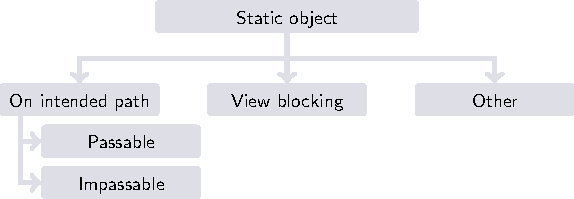
\includegraphics{figures/static_object}
	\caption{Tags that describe a static object.}
	\label{fig:tree static object}
\end{figure}

%\Cref{fig:tree crossing vehicle} describes whether a crossing road user has priority or not. If there is no crossing actor in the scenario, then the tag is not applicable (N.A.). Note that a crossing actor can refer to any type of traffic participant, e.g., a vehicle or a VRU. Although the tags mention actors, the rules of priority, or traffic rules in general, are related to the road layout and consequently these tags are considered part of the static environment.\\
%
%\begin{figure}
%	\centering
%	\tree{Crossing actor}{Ego priority; Actor priority; N.A.}
%	\caption{Tags indicating priority in case of crossing actors.}
%	\label{fig:tree crossing vehicle}
%\end{figure}

\subsubsection{Traffic light}
\label{sec:traffic light}

For a traffic light, we consider the tags ``Red'', ``Amber'', ``Green'', and ``N.A.``. The last tag is applicable in case the traffic light is not operating.
%\Cref{fig:tree traffic light} presents the tags that refers to the traffic light status that is applicable for the ego vehicle. If physically a traffic light is present, but the traffic light is not operating, the tag ``N.A.'' is applicable. 
Note that it might be possible that multiple tags are applicable for a scenario. For example, if the traffic light is initially green and turns amber during the timespan of the scenario, both the tags ``Amber'' and ``Green'' are applicable.

%\begin{figure*}[t]
%	\centering
%	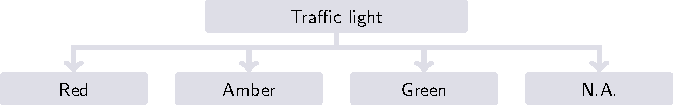
\includegraphics{figures/traffic_light}
%	\caption{Tags that describe the traffic light status for the ego vehicle.}
%	\label{fig:tree traffic light}
%\end{figure*}



\subsection{Tags for the conditions}
\label{sec:conditions}

Separate tags are specified to describe weather and lighting conditions. Weather and lighting conditions are possibly important in the specification of the operational design domain (ODD) of an AV. It might be indicated by an AV developer that the ODD does not include heavy rain or dark night conditions in the absence of street lights. \Cref{fig:conditions} shows tags describing the weather condition (based on \cite{mahmassani2012use}). Tags need to be as specific and quantifiable as possible. Consequently, definitions according to meteorology are followed. 

Tags for different lighting conditions are based on \cite{golob2003relationships}, see \cref{fig:conditions}. Although it might seem straightforward to use the lux level as a quantitative measure for the lighting condition, in this paper, we choose to use a qualitative description, relating the light level to the time of day and the possible presence of artificial lighting. In a study into the influence of ambient lighting conditions on the detection of pedestrians by Automated Emergency Braking systems \autocite{wouters2013influence}, it appeared that lux levels show large variations on the public road. 
The light conditions were measured at a typical junction equipped with street lights during night time. Variations with a factor of 100 to 1000 easily occur due to changes in position underneath a street light. 
Also the presence of other ambient lighting sources has a large influence. As it is not possible to indicate an average lux level, we use a qualitative description of the light level. 
During daytime, there is a strong relation between the weather condition and the available light in a scenario. These weather conditions have been included in the tag tree for lighting.
Glare, a bright and strong light that shines directly onto the ego-vehicle's camera, is another important lighting condition influencing an AV's performance. Glare can be caused by the sun shine while driving to the West just before sunset (or to the East just after sunrise), or by cars in on-coming traffic using high beam headlights. A branch on glare has been added to the lighting tree.  

\begin{figure*}[t]
	\centering
	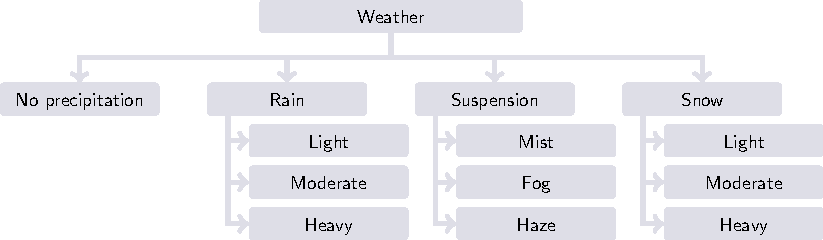
\includegraphics{figures/weather}\\
	\vspace{0.5em}
	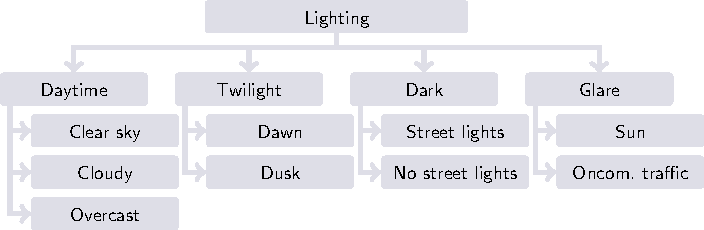
\includegraphics{figures/lighting}
	\caption{Tags for weather condition, based on \cite{mahmassani2012use} and lighting conditions, see \cite{golob2003relationships}.}
	\label{fig:conditions}
\end{figure*}
